\section{Studien zur Browserkompatibilität}
\label{sec:studien-zur-browser-kompatibilitaet}

Im \autoref{sec:browserprodukte} wurde die Anzahl an Studien zur Browserkompatiblität dargestellt. Dabei wurde in der Suche jeweils bei den Optionen \texttt{von} und \texttt{bis} des Erscheinungsjahres jedes Jahr einzeln eingegeben und eine Suche durchgeführt, die Trefferanzahl wurde dann notiert. Die Daten hierfür wurden über die Literatursuchmaschine \enquote{Google Scholar} am 25.02.2021 abgerufen. Für die Suche wurde folgender Suchterm benutzt:
\begin{verbatim}
"cross browser" compatibility|incompatibility|inconsistency|XBI
\end{verbatim}

\begin{wraptable}[10]{r}{0.42\linewidth}
\centering
\vspace{-\baselineskip}
\begin{tabular}{|l|l|}
  \hline
  Jahr & Suchtreffer \\
  \hline
  2015 & 272 \\
  \hline
  2016 & 228 \\
  \hline
  2017 & 208 \\
  \hline
  2018 & 204 \\
  \hline
  2019 & 172 \\
  \hline
  2020 & 167 \\
  \hline
\end{tabular}
\caption{Suchtreffer zu Studien über Browserkompatibilität}
	\label{tab:suchtreffer-metastudie}
\end{wraptable}

\def\lc{\left\lceil}   
\def\rc{\right\rceil}

Die jahresbezogene Trefferanzahl (vgl. \autoref{tab:suchtreffer-metastudie}) soll aufdecken, ob ein Trend in der Literatur zu erkennen ist. Ein schwacher, aber vorhandener Negativtrend konnte festgestellt werden.

Weiterhin lässt sich die selbe Thematik bei Google Trends \cite{GoogleTrendsCrossBrowserCompatibility} untersuchen. Hierbei wurden die Suchtrends für den Suchterm \texttt{cross browser compatability} abgerufen und geplotted (vgl. \autoref{fig:google-search-trends_cross-browser-compatability}). Dabei lässt sich ebenso ein Negativtrend erkennen.

\begin{figure}[H]
	\centering
	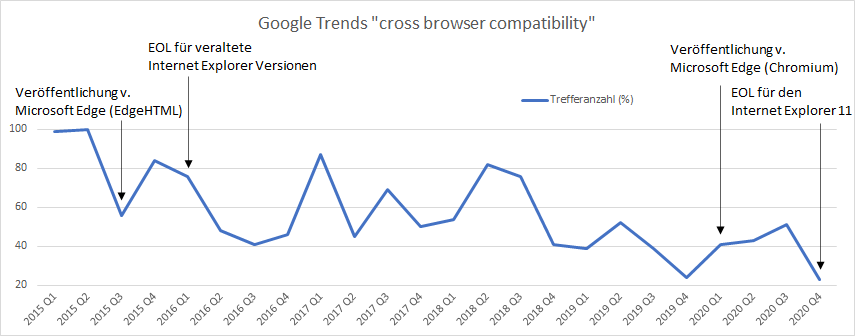
\includegraphics[width=0.84\linewidth]{img/99_postscript/google-trends_cross-browser-compatability.png}
	\caption{Google Trends zur Browserkompatibilität, angereichert mit \cite{MicrosoftIEandEdgeLifecycleFAQ}}
	\label{fig:google-search-trends_cross-browser-compatability}
\end{figure}
